%%%%%%%%%%%%%%%%%%%%%%%%%%%%%%%%%%%%
% template.tex
%
% Template for the KTHEEposter class.
%
% Original version: Mats Bengtsson, 28/5 2002
% Updated:
%   Mats Bengtsson April 2011 - July 2012
%   Manuel Olguín October 2018
%%%%%%%%%%%%%%%%%%%%%%%%%%%%%%%%%%%%

%\PassOptionsToPackage{showframe}{geometry}
\documentclass[portrait, a1]{KTHEEposter}
\usepackage{lipsum}
\usepackage{listings}
\usepackage{enumitem}
\usepackage[format=hang]{caption}
\usepackage{subcaption}
\captionsetup{font=normalsize,labelfont={bf,sf}}
\captionsetup[sub]{font={small}, textfont={normalfont}, labelfont={bf,sf}}
\usepackage{indentfirst}
\lstset{basicstyle=\ttfamily, frame=single}
\usepackage{pgfplots}
\pgfplotsset{compat=1.14}
\usepackage[export]{adjustbox}
\usepackage{tikz}
\usetikzlibrary{shapes,arrows.meta,positioning,automata}
\usepackage{sourcecodepro}
\usepackage{todonotes}
\usepackage{wrapfig}

\usepackage[style=ieee,
backend=bibtex,
sorting=none,
sortcites,
maxbibnames=1,
minbibnames=1,
maxcitenames=2, 
mincitenames=1]{biblatex}
\AtBeginBibliography{\footnotesize}
\addbibresource{bibliography.bib}


\kthlogo{kth_eng_cmyk}
\extralogo{img/cmu_csd_logo}
\kthcolor{KTHblue}

\begin{document}
    
    \title{\LARGE\bfseries Scaling on the Edge:\\A Benchmarking Suite For Human-in-the-Loop Applications}
    
    \author{\Large Manuel Olguín, Junjue Wang,\\Mahadev Satyanarayanan, James Gross}
    \maketitle
    
    \begin{pcolumns}[3]
        \begin{pcolumn}[2]
            \begin{pframe}[.7]
                \section{Abstract}
                Benchmarking human-in-the-loop applications running on edge computing infrastructure is complex given their nature, which heavily depends on the actions taken by the human user.
                This limits reproducibility as well as feasibility of performance evaluations.
                We propose a methodology and present a benchmarking suite that can address these challenges.
                Our core idea rests on recording traces of these applications which are played out in a controlled fashion based on an underlying model of human behavior.
                The traces are exposed to the original backend compute process of the respective human-in-the-loop application, generating realistic feedback.
                This allows for an automated system which greatly simplifies benchmarking large scale scenarios.
            \end{pframe}
            \begin{pframe}[1.3]
                \section{Basic Idea}
                \begin{itemize}
                    \item Benchmarking human-in-the-loop applications is \textbf{hard} due to human users:
                    \begin{itemize}
                        \item They are unpredictable.
                        \item They make scaling difficult (you need more of them!).
                    \end{itemize}
                    \item What if we could cut out the user?
                \end{itemize}
                \medskip
                \begin{center}
                    \medskip
                    \makeatletter
                    \let\theoldfigure=\fnum@figure
                    \renewcommand{\fnum@figure}{Step~\thefigure}
                    \makeatother
                    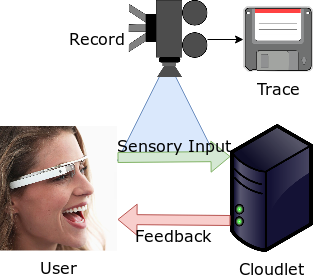
\includegraphics[width=.75\linewidth]{img/trace_idea_1}
                    \captionof{figure}{Trace user input while operating the target application.}
                    
                    \medskip\medskip
                    
                    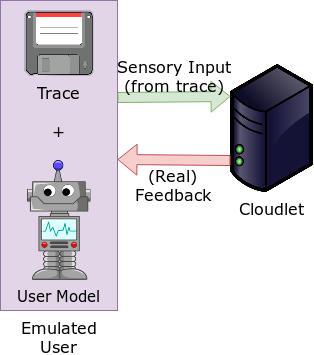
\includegraphics[width=.75\linewidth]{img/trace_idea_2}
                    \captionof{figure}{Replace user with recorded trace plus a user model.}
                    \makeatletter
                    \renewcommand{\fnum@figure}{\theoldfigure}
                    \makeatother
                    \setcounter{figure}{0}
                \end{center}
                
            \end{pframe}
        \end{pcolumn}%
        \begin{pcolumn}[2]
            \begin{pframe}[1.52]
                \section{Design \& Implementation}
                \begin{center}
                    \medskip
                    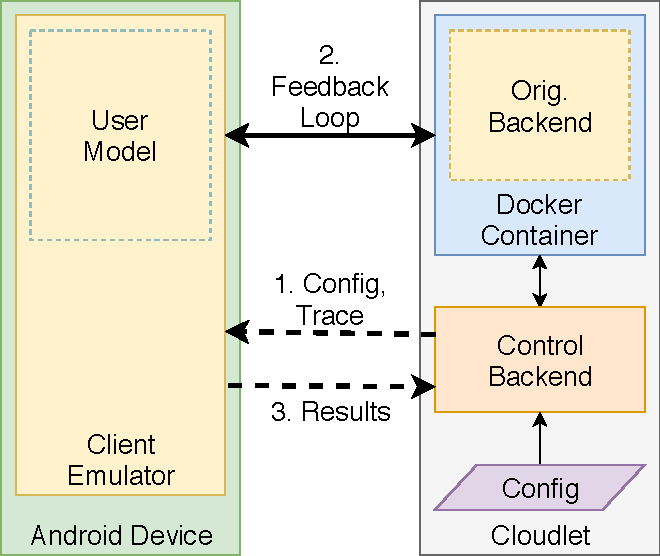
\includegraphics[width=.85\linewidth]{img/TraceReplay_GenArch}
                    \captionof{figure}{Suite Architecture}
                    \medskip
                \end{center}
                \begin{itemize}
                    \item The \emph{control backend} controls the experiments and collects measurements from the application and the cloudlet itself.
                    \item The \emph{client emulators} play out a prerecorded sensory input trace over the network in a controlled fashion, while collecting client-side metrics.
                \end{itemize}
            %\end{pframe}%
            %\begin{pframe}[1.13]
                \begin{center}
                    \medskip
                    \adjustbox{scale=0.7}{
    \ttfamily\centering%\fbox{%
    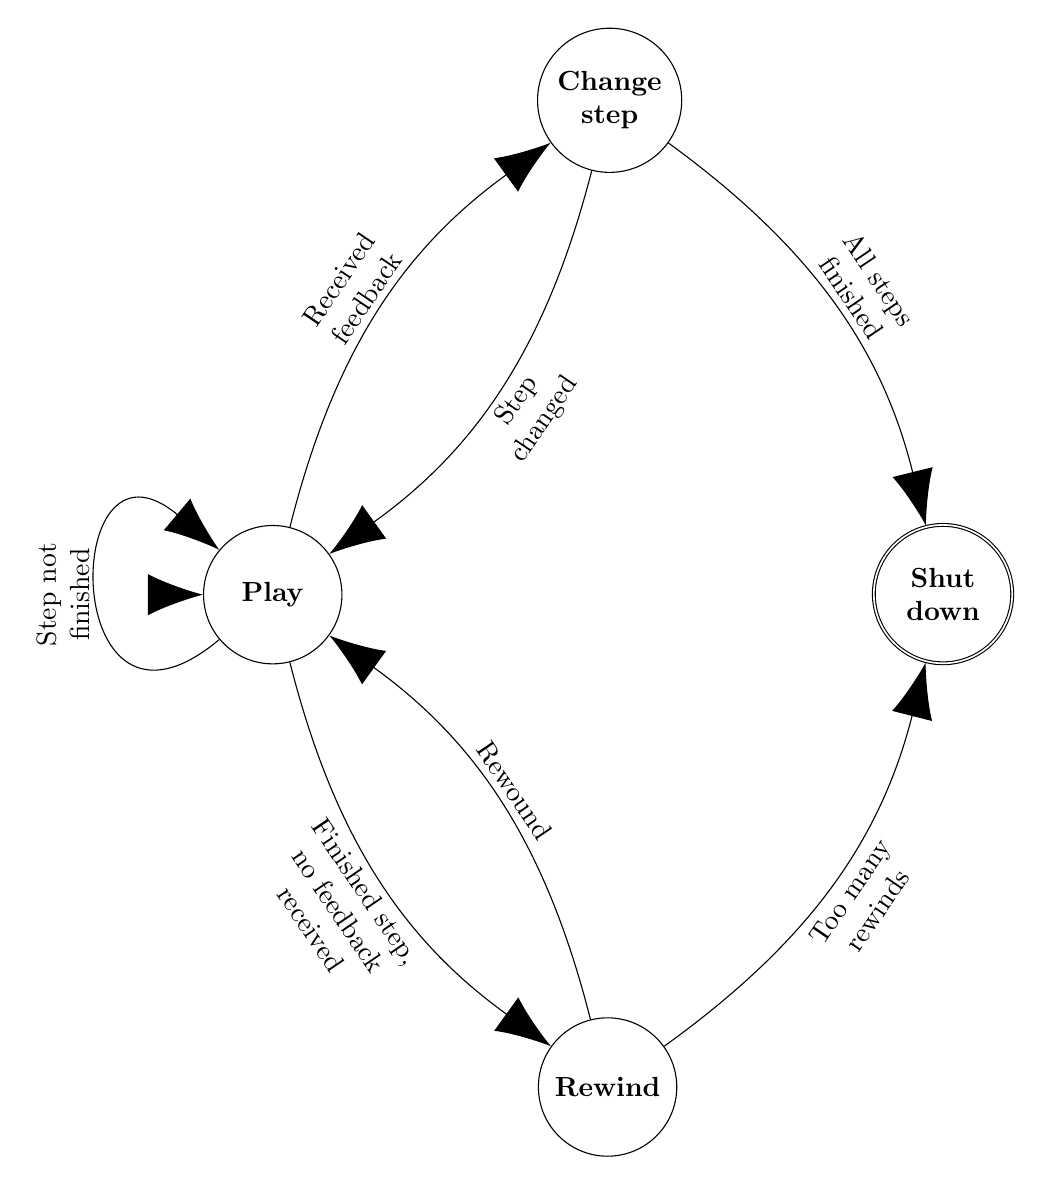
\begin{tikzpicture}[align=center,
        node distance=5cm and 3cm,
        every initial by arrow/.style={-{Latex[length=7mm]}}]
        % Place nodes              
        \node [initial, state, minimum size=5em, initial text=] (play) {\textbf{Play}};
        \node [state, above right=of play, minimum size=5em] (change) {\textbf{Change}\\\textbf{step}};
        \node [state, below right=of play, minimum size=5em] (rewind) {\textbf{Rewind}};
        \node [state, accepting, above right=of rewind, minimum size=5em] (shutdown) {\textbf{Shut}\\\textbf{down}};

        % Draw edges
        \path[draw, -{Latex[length=7mm]}, sloped, anchor=center]
        (play) edge [bend right=20] node[below] {Finished step,\\no feedback\\received} (rewind)
        edge [bend left=20] node[above] {Received\\feedback} (change)
        edge [in=140, out=220,looseness=6] node[above] {Step not\\finished} (play)

        (change) edge [bend left=20] node[below] {Step\\changed} (play)
        edge [bend left=20] node[above] {All steps\\finished} (shutdown)

        (rewind) edge [bend right=20] node[above] {Rewound} (play)
        edge [bend right=20] node[below] {Too many\\rewinds} (shutdown);

    \end{tikzpicture}
}%}
                    \captionof{figure}{Simple user model used for the initial iteration of the suite.}
                    \medskip
                \end{center}
                
                We implement a very simple user model in order to be able to react to feedback from the application and adapt our replay of the trace to the current system conditions.
                %We plan to fully parameterize the components of this model in the future, in order to be able to construct more realistic user models.
            \end{pframe}%    
            \begin{pframe}[.48]
                \section{Demo}
                The client emulators in particular will be showcased in the \textsc{demo}.
                We will demonstrate the workings of the system on a simple LEGO task assistance application, and spectators will be able to follow the replay of the trace as well as the behavior of the user model through the client devices.
                \medskip
                \begin{center}
                    \medskip
                    
\includegraphics[width=.5\textwidth]{img/lego}%
                \end{center}
            \end{pframe}    
        \end{pcolumn}%
        \begin{pcolumn}[3]
            \begin{pframe}[2.14]
                \section{Some Example Results}
                \begin{center}
                    \medskip
                    
\includegraphics[width=\linewidth]{plots/comparison/box_legend.pdf}
                    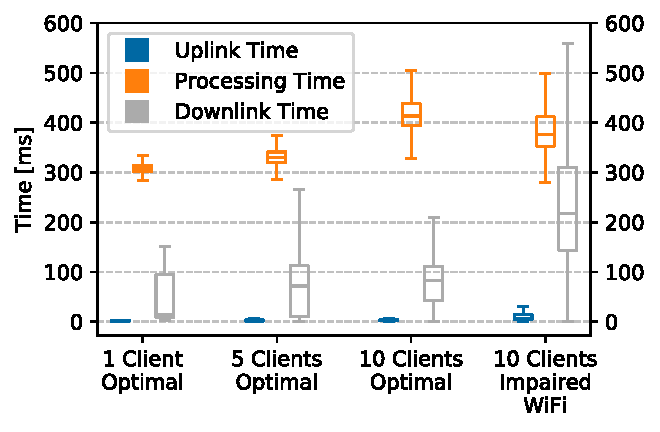
\includegraphics[width=\linewidth]{plots/comparison/box_feedback.pdf}
                    \captionof{subfigure}{Inputs that triggered feedback.}
                    \medskip
                    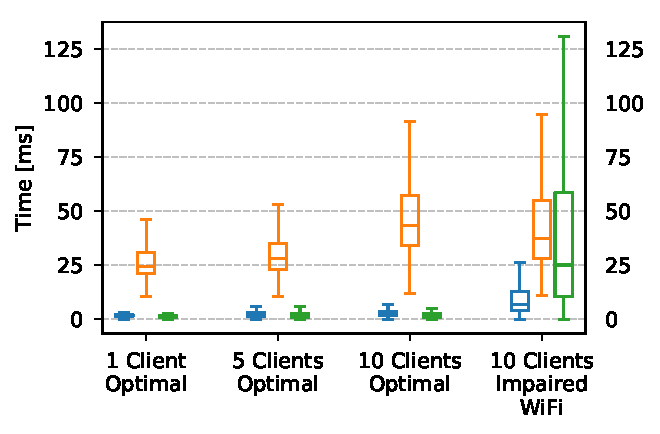
\includegraphics[width=\linewidth]{plots/comparison/box_nofeedback.pdf}
                    \captionof{subfigure}{Inputs that did not trigger feedback.}
                    \captionof{figure}{Comparison of the latency distributions across system components for a series of scenarios.}
                    \medskip
                \end{center}
            
                 These results could be useful for:
                 \begin{itemize}
                     \item System designers wishing to identify bottlenecks in their hardware stack.
                     In this case, they could determine that the wireless link seems to be the weak point when the connection is not optimal.
                     \item Application developers who want to find potential for optimization in their applications.
                 \end{itemize}
            \end{pframe}
            \begin{pframe}[.17]
                \medskip\itshape\footnotesize
                We will eventually make the benchmark suite available as Free and Open Source Software.
                The traces will also be made available under a Creative Commons License.
            \end{pframe}    
            \begin{pframe**}[.69]
                \nocite{*}
                \small
                \printbibliography
            \end{pframe**}
        \end{pcolumn}
    \end{pcolumns}
    
\end{document}